\chapter{配管データセット}

前章では,アイソメ図を作成するためのネットワーク構造を提案した。
本章では、深層学習に用いるデータセットの収集及び、作成方法について論じる。


\section{使用機材}
データセットの取得にはRGB-Dカメラを使用する。従来の方法ではLIDARセンサーを用いて配管3Dデータやアイソメ図を作成していた。
しかし、LIDARセンサーは高価であり、一般的に使用することが困難であるという欠点を抱えていた。そのため、RGB-DカメラはLIDARセンサーよりも比較的安価であるため本研究のデータセット収集に使用する。\\
次に、RGBカメラではなくRGB-Dカメラを使用する利点を3点紹介する。まず、一つ目にRGB-Dカメラはカラー画像だけでなく距離情報を取得できるという点である。
配管のアイソメ図には配管のそれぞれの部位の長さを正確に示す必要がある。そのため、RGB画像には距離情報が含まれていないことからスケールを必要とする際にはDepth画像が重要になるのだ。\\
二つ目に照明などの光の明暗に影響されない点である。図3.2よりRGB画像は撮影する環境が照明が無く暗闇だった場合、撮影された画像には認識したいオブジェクトの特徴を捉えることは困難である。これはRGB画像が光に反射された物体の度合いを数値化しているため、極端に明るすぎたり
暗すぎるとRGB画像が活用できなくなる。特に配管が設置されている地盤地下や天井裏などの照明を当てることが困難な環境ではDepth画像が必要になる。\\
\begin{figure}[htbt]
    \centering
     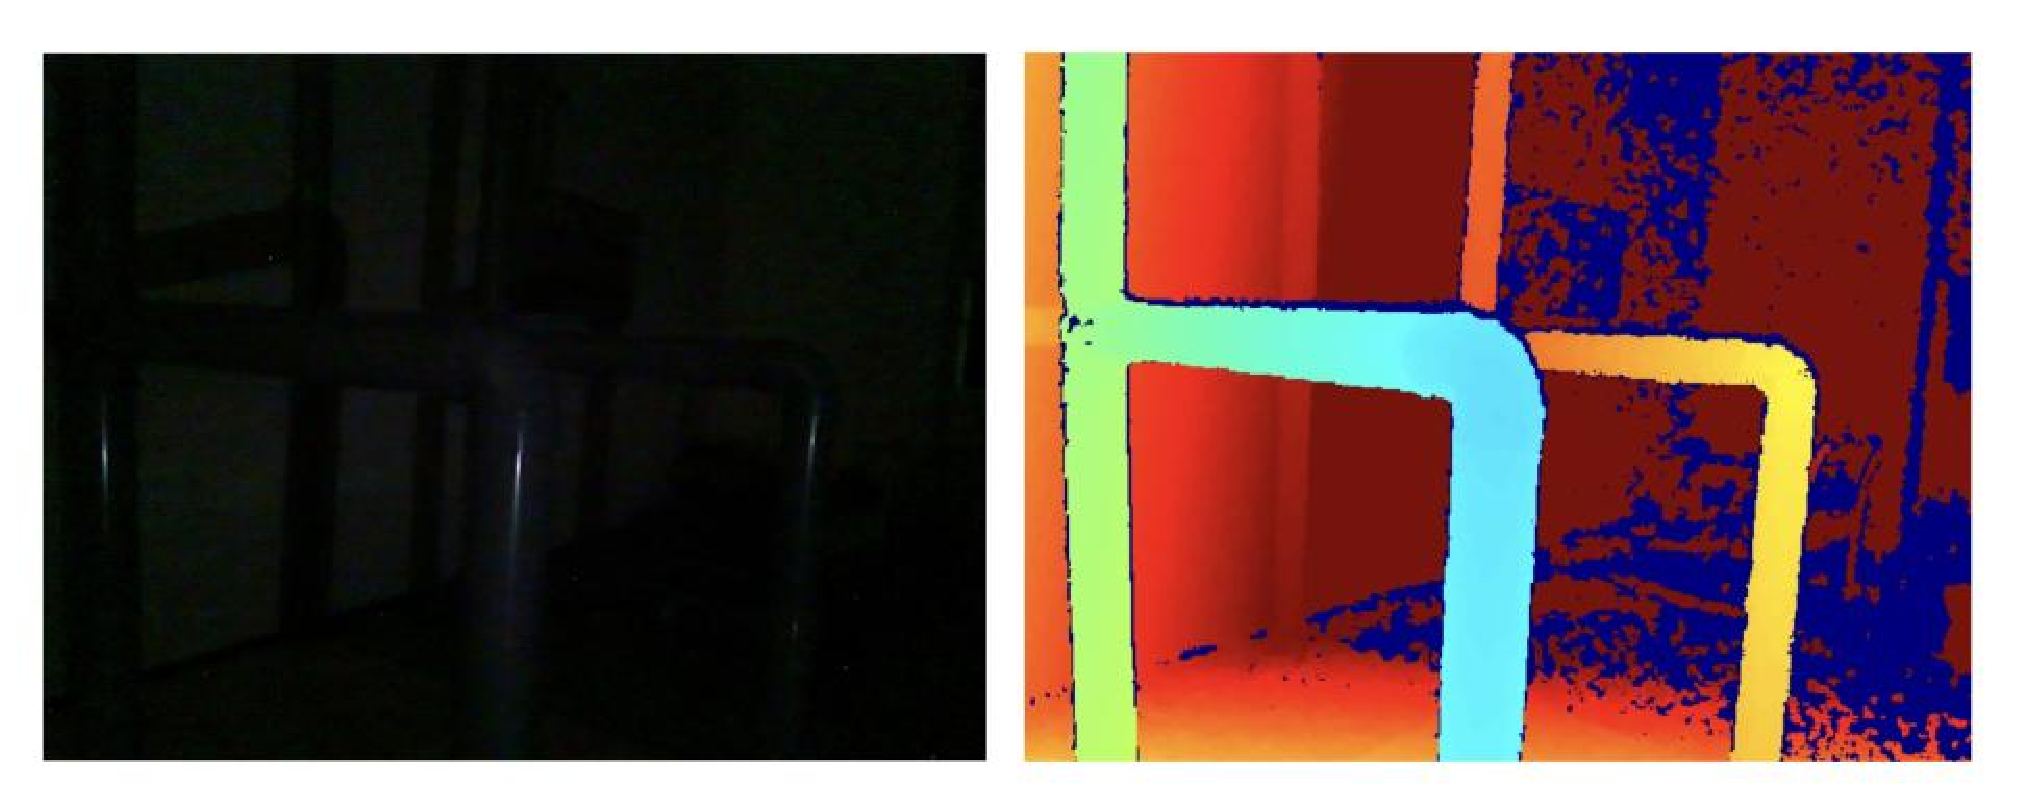
\includegraphics[height=55mm]{pipe_rgbd.eps}
     \caption{暗所でのRGB-Dカメラの撮影}
     \label{fig:f2}
\end{figure}

三つ目に配管が背景色と同様の色を示していた場合に、区別が容易に可能であるという点である。RGB画像では色の違いの判断が難しいが、Depth画像は距離情報の違いを示すことができるため、
背景と異なる物体として認識可能になる。配管の場合、壁と配管の色に差異が生まれにくいことが多々あるためDepth画像を使用するメリットになる。また、配管が重なり合った場合にも前後関係が区別しない場合にも効果を発揮する。\\

カメラはインテル社製のIntel Realsense L515を使用した。Realsense L515を使用した理由はRealsenseカメラの中でも屋内に適したRGB-Dカメラであるからだ。このカメラは外光の影響を受けやすいが、
屋内の環境であればその影響を受けないため、配管などの室内で多く使用される環境では非常に適していると判断した。
\begin{figure}[htbt]
    \centering
     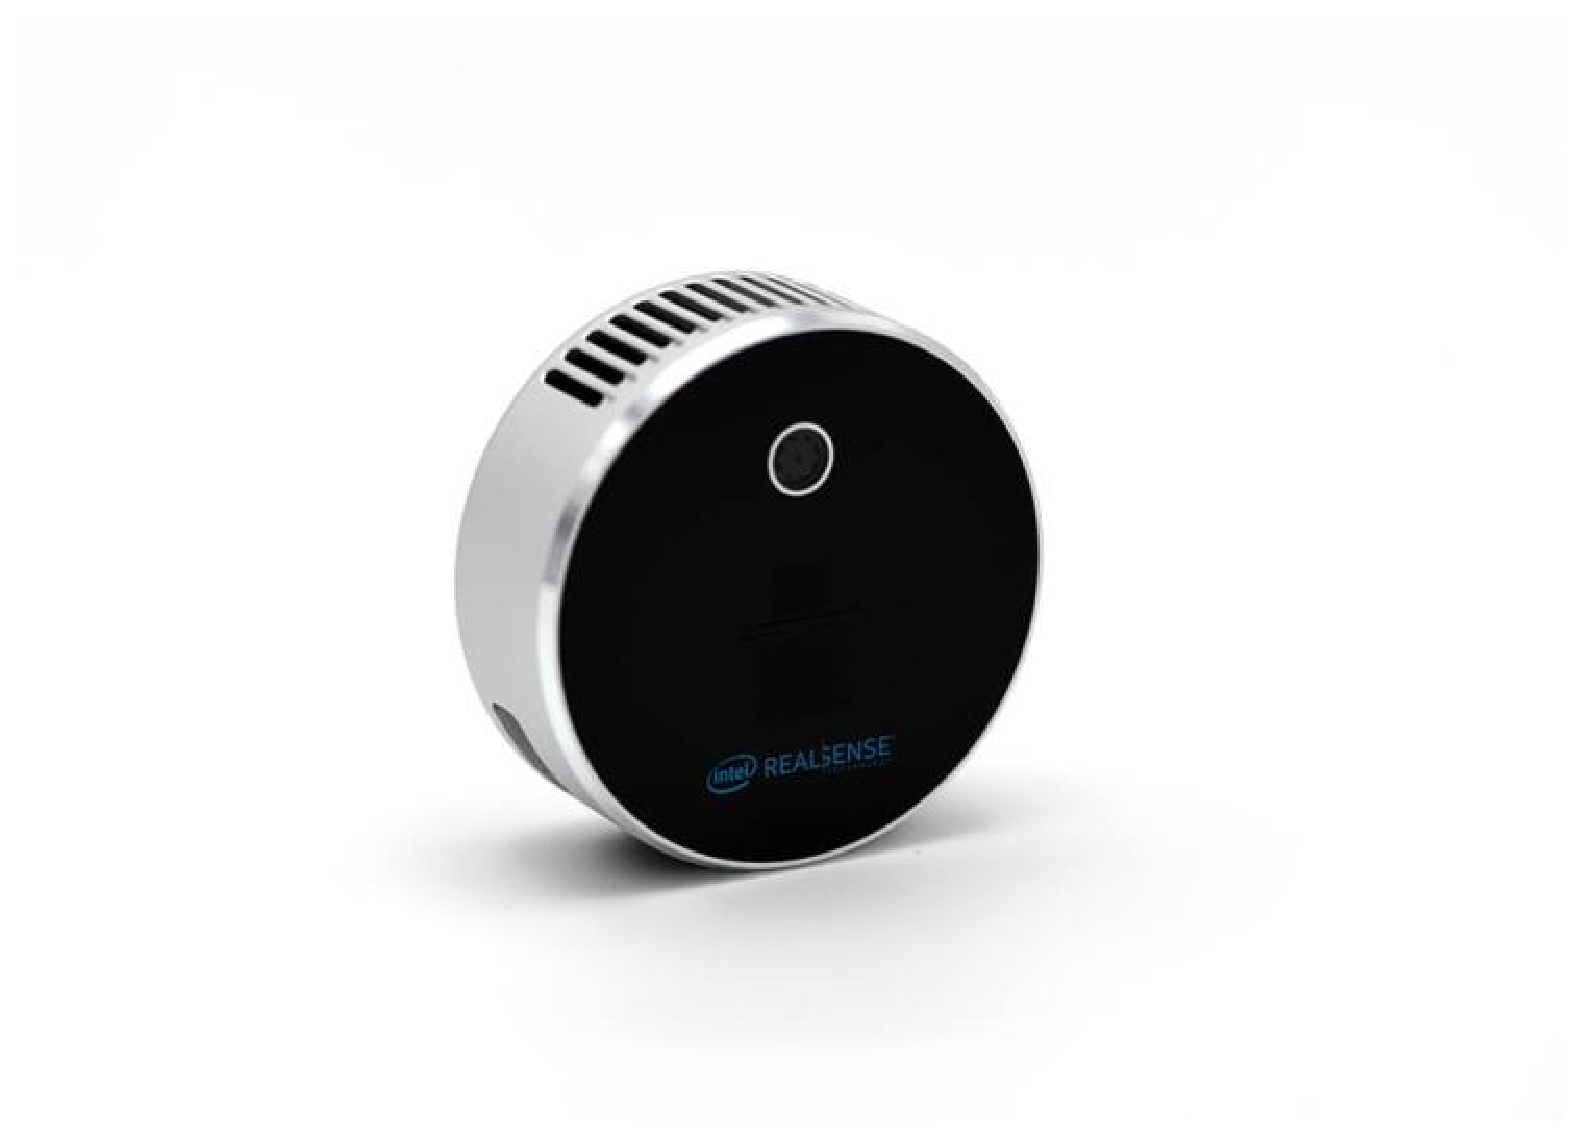
\includegraphics[height=55mm]{realsense.eps}
     \caption{Intel Realsense L515}
     \label{fig:f2}
\end{figure}

しかし、Realsense L515は仕様上、RGBカメラとDepthカメラの位置が異なるため、撮影した際に両方の画像を比較すると画角に差異が生じてしまう。これは、データセットのラベリングを行う際に配管のピクセル座標に
それぞれの画像で異なると認識の精度に大きな誤差が生じてしまう。そのため、Realsenseのalignmentライブラリを使用する。これによって両方のカメラの画角をソフトウェア上で位置合わせが可能になる。

\section{物体検出のデータセット収集}
深層学習による認識ネットワークにはデータセットの数量が多いほど精度とロバスト性が向上する。
それは様々な場面での配管の写真を学習することによってどの環境においても対応できる汎用性が高まることを意味している。本研究使用するデータセットの一部を図3.2に示す。
配管には曲管やT字管や直管が含まれており、この画像内の中から曲管とT字管を全て認識できることを目標とする。また、Depth画像の有効性を示すためにテスト画像では
暗闇の中に配管を設置したデータセットを用意した。Depth画像は光の影響を受けにくいことから、暗闇の中でも配管を認識できるかを検証する。\
収集したデータはラベリング作業を行う。これは深層学習するにおいての正解データとして、予め画像内のどの部分が曲管又はT字管であるかをアノテーションする必要がある。
本研究では配管画像に対して曲管、T字管の二つのクラスに分けてラベリング作業を行った。

\begin{figure}[htbt]
	\centering
	 \includegraphics[height=155mm]{imges.eps}
	 \caption{学習に用いるデータセットの例}
	 \label{fig:f2}
\end{figure}

\section{6D姿勢推定のデータセット収集}
6D姿勢推定のデータセットにはColmapを使用して点群データを取得する。Colmap2D画像から点群を再構築するために使用されるソフトウェアである。
この2D画像は異なる視点から撮影された同じオブジェクトの画像を複数枚利用することで3次元情報を復元することができる。
そのため、本研究では曲管とT字管の周囲をそれぞれ撮影し、Colmapを使用することで点群データを取得した。
しかし、点群データを取得してもColmapで生成されたデータには距離情報が含まれていないため、別途Depth画像を使用してアイソメ図作成の際に使用しなければいけない。
\begin{figure}[htbt]
	\centering
	 \includegraphics[height=95mm]{bent.eps}
	 \caption{Colmapを用いた曲菅の点群データ}
	 \label{fig:f2}
\end{figure}

\begin{figure}[htbt]
	\centering
	 \includegraphics[height=100mm]{junction_p.eps}
	 \caption{Colmapを用いたT字管の点群データ}
	 \label{fig:f2}
\end{figure}